\documentclass[french]{report}
\usepackage[utf8]{inputenc}
\usepackage[T1]{fontenc}
\usepackage{babel}
\usepackage[autolanguage]{numprint}
\usepackage[backend=bibtex]{biblatex}
\usepackage{csquotes}
\addbibresource{mabib.bib}
\usepackage{graphicx}
\usepackage{wrapfig}
\usepackage{lipsum}
\usepackage{float} 
\usepackage{multirow}

\begin{document}

\begin{titlepage}
    \begin{center}
        \LARGE \textbf{Photo-z estimation by Deep learning}\\
        \large \textit{<<Aproach by images>>}
    \end{center}
    
    \begin{center}
        \Large \textbf{Présenté par:} \textit{Ousmane Issa}\\
        \Large \textbf{Sous la direction de:} \textit{  Pr. Engelbert Mephu Nguifo}
    \end{center}
\end{titlepage}

\tableofcontents


\section*{\textit{Résumé:}}

\section*{\textit{Abstract:}}


\chapter*{Introduction}
Après avoir introduit, le contexte du problème est détaillé, il est suivi par la motivation.


\part{Photo-z estimation by Deep learning \\
        \large \textit{<<Aproach by images>>}}

\section*{Décalage vers le rouge (Redshift)}
Le redshift est l'augmentation de la longueur d'onde d'un objet lors de l'application de radiation électromagnétique sur cet objet. Un observateur peut remarquer le déplacement de la lumière de cet objet vers le rouge, ce qui est un effet contraire au blueshift (décalage vers le bleu) où l'observateur remarque le déplacement de la lumière de l'objet vers le bleu.
\begin{figure}[H]
	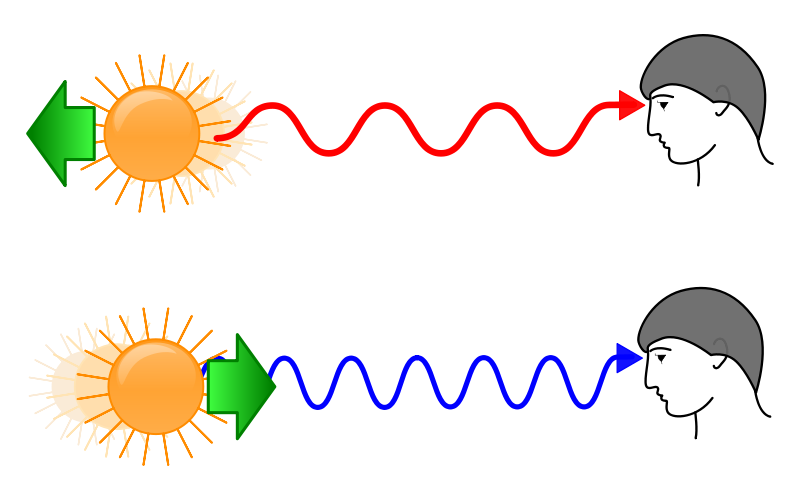
\includegraphics[scale=0.3]{images/reshift.png}
	\caption{illustration du redshift et blueshift}
	\label{redblue}
\end{figure}
Le reshift est noté $z$ et se manifeste quand l'objet en mouvement tout en s'éloignant de l'observateur (effet dopler) ou il est du à l'expansion de l'univers (redshift cosmologique) ou due à la gravitation (redshift gravitationel). Dans notre cas le redshit qu'on essaie d'estimer correspond au redshift cosmologique et il s'obtient de la manière suivante: $1 + z = \frac{\lambda_{observé}}{\lambda_{emis}}$ où $\lambda_{observé}$ et $\lambda_{observé}$ sont respectivement la longueur d'onde observée et celle émise. La loi de Huble établit une relation entre la distance et le redshift cosmologique comme suit $v = H_0d = cz$ où $d$ est la distance, $v$ la vitesse, $c$ la vitesse de la lumière, $H_0$ la constance de Huble et $z$ le redshift cosmologique.
%\section*{Calcul du redshift}
%Nous avons deux manières de calculer le redshift, une méthode dite exacte (spectroscopie) qui donne une bonne estimation du redshift et une autre qui ne permet que de donner une estimation du redshift (photométrie). 
\section*{Spectroscopique}
La méthode spectroscopique mesure le redshift par la dispersion de la lumière en comparant le décalage entre les lignes spectrales des éléments chimiques émises et celles absorbées. La spectroscopie donne des estimations précises du redshift, néanmoins elle est couteuse et prend beaucoup de temps. Ce qui encourage les scientifiques à chercher d'autres moyens moins couteux pour estimer le redshift.
\begin{figure}[H]
	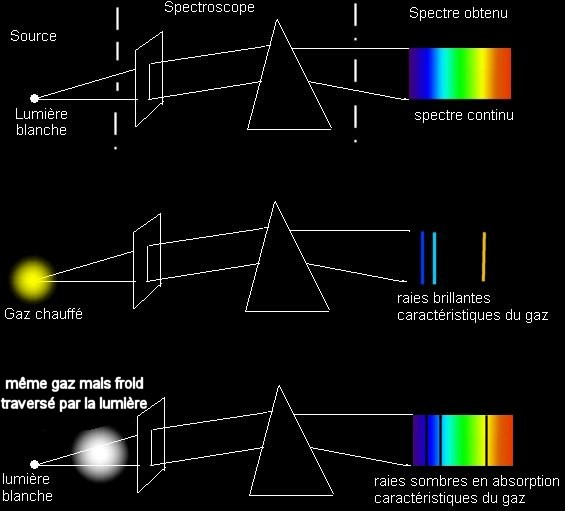
\includegraphics[width = 13cm, height = 5cm]{images/spectroscopie.jpg}
	\caption{Expériences spectroscopiques}
	\label{spec}
\end{figure}   
\section*{Estimation par photométrie}
La méthode basée sur la photométrie utilise un ensemble de filtres profonds dans des longueurs d'ondes spécifiques (5 bandes dans notre cas) pour capturer certaines caractéristiques de l'objet concerné. Puisque c'est une opération rapide, la photométrie donne une grande quantité d'observations en terme de nombre et de profondeurs de caractéristiques de chacune des observations. À partir des caractéristiques de l'objet observé, on tente de déterminer son décalage vers le rouge. Donc la précision du calcul du redshift par données photométries dépend de la profondeur du mesure de ces caractéristiques. SDSS a collecté plus de 300 millions des objets photométries. Le télescope LSST (Large Scale Survey Telescope) qui sera bientôt déployé donne plus de caractéristiques que ceux existants (utilise 6 bandes allant de l'ultra violet à l'infra-rouge), qui va rendre plus précis l'estimation du redshift par photométrie. Dans ce travail nous essayons d'estimer directement le redshift à partir des images.

\begin{figure}[H]
	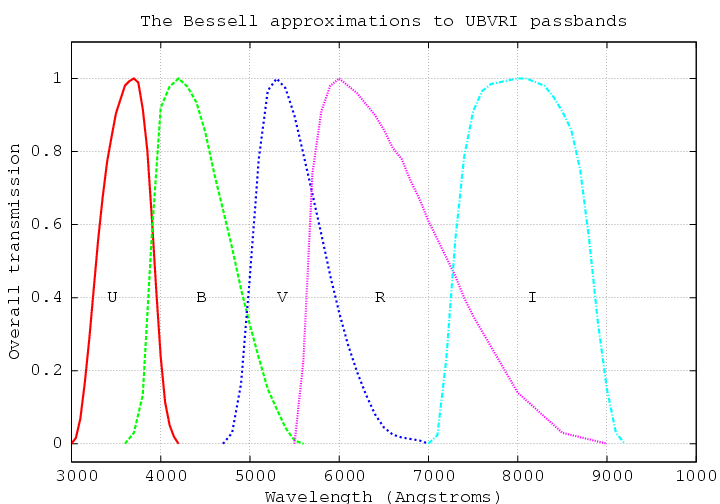
\includegraphics[width = 13cm, height = 5cm]{images/photometrie.png}
	\caption{Expériences photométries}
	\label{photo}
\end{figure}

Ces derniers années plusieurs  travaux \cite{Gabriel, meuphirim, isanto, photoSED, stack} ont été fait à partir des données photométries pour l'estimation du redshift. La méthode d'estimation du redshift par données photométries est divisée en deux sous méthodes à savoir celle basée modèle et celle basée sur les techniques de l'apprentissage automatique et statistiques dite empirique. Ces deux sous-méthodes seront détaillées dans le chapitre 1.

\section*{Qualité de prédiction du redshift}
Il existe plusieurs paramètres pour définir la qualité de prédiction du redshift, ils sont tous basé sur une fonction de perte normalisée (erreur normalisée). L'objectif de ce travail est de trouver une fonction ($f$) qui prend en entrée des images superposées dans 5 bandes de longueurs d'onde différentes d'un corps cosmologique et retourne le redshift correspondant. Pour cela une fonction ($\Delta z$) dite fonction d'erreur est définie, elle permet de vérifier si la fonction $f$ prédit bien en générale le redshift d'un corps en faisant la soustraction entre la valeur exacte du redshift (valeur spectroscopique) et celle prédite(estimée) $\Delta z = z_{phot} - z_{spec}$. L'erreur normalisée est définie comme suit: \\
$\Delta z_{norm} = \frac{\Delta z}{z_{spec} + 1}$ \\
Dans ce travail nous utilisons principalement quatre paramètres de mesure de qualité de prédiction du redshift: \\
\begin{itemize}
	\item Le biais qui est la moyenne de l'ensemble des erreurs notée %$\mu(\Delta z)$ ou
	 $\mu(\Delta z_{norm})$ pour l'erreur normalisée. \\ %$\mu(\Delta z) = \frac{\sum_{i=1}^{n} \Delta z_i}{n}$ et
	 $\mu(\Delta z_{norm}) = \frac{\sum \limits_{i=1}^{n} \Delta z_{norm_i}}{n}$
	\item Le standard déviation noté $\sigma (\Delta z_{norm}) = \sqrt{\frac{\sum \limits_{i = 1}^{n} (\Delta z_{norm_i} - \mu(\Delta z_{norm}) )^2}{n}}$ 
	\item La proportionnalité des outliers/particuliers catastrophiques mesurée par $(\frac{card(|\Delta z_norm| \geq 0.15)}{n})*100$ ou $(\frac{card(|\Delta z_norm| \geq 3\sigma(\Delta z_norm))}{n})*100$ en pourcentage. 
	\item  Erreur moyenne quadratique (RMSE) qui est similaire à la déviation standard.
	$RMSE = \sqrt{\frac{\sum \limits_{i=1}^{n} (\Delta z_{norm_i})^2}{n}}$. \\
	Où $n$ est le nombre total de l'échantillon de test, et $card$ est la fonction cardinale.
\end{itemize}


\chapter{Travaux existants dans la littérature}
\section{Méthodes basées sur les modèles (template-based)}
Ces méthodes sont basées sur de modèles prédéfinis utilisant la distribution spectral de l'énergie. Elles supposent un ensemble de modèles de galaxies et tire le modèle le plus adapté et ensuite deduire le redshift \cite{Narciso, Gabriel, photoSED}.\\ 
Cette méthode de mesure du redshift est biaisée (seulement les galaxies) et ainsi entraîne des erreurs dans la prédictions des erreurs. À partir de template-based on peut déterminer d'autres composants physiques que le redshift \cite{meuphirim}. Plusieurs tentatives de l'amélioration de la précision du redshift de galaxies ont été faites, ci-dessous un tableau des certains travaux intéressants de la littérature.
\begin{table}[!ht]
\centering    
\begin{tabular}{|c|c|c|c|c|c|}
    \hline paper & database & type/SED TEMP & $\mu(Z_{norm})$ & $std(Z_{norm})$ & $|Z_norm|\ge0.15 (\%)$\\
    \hline 
    \multirow{2}{1cm}{\cite{sql}} & PHAT & GALAXY/LP Flat Err & 0.0013 & 0.0445 & 9.88  \\
    \cline{2-6}
     & CAPR & Galaxy/LP HDF Err & -0.0081 & 0.0490 & 7.65\\
    \hline
    \multirow{2}{1cm}{\cite{Narciso}} & \multirow{2}{1cm}{HDF} & GALAXY/BPZ & 0.08 & &  \\
    \cline{3-6} 
     &  & Galaxy/ML & 0.10 &  & \\
    \hline
    \cite{photoredSDSS} & SDSS DR12 & GALAXY & 0.0000584 & 0.0205& 4.11\\
    \hline
    
    
    
    %&  \\
    %& 
\end{tabular}
    \caption{Résultat concernant la méthode basée modèle}
    \label{base_model}
\end{table}

Dans \cite{Narciso} deux modèles probabilistes ont été utilisés: maximum likelihood (ML) et le modèle bayesian (BPZ). 

Dans \cite{sql}, l'analyse est faite directement sur les différentes bases de données sans les déplacer. Cela permet non seulement d'éviter un télé-chargement long des données et l'obligation d'avoir un très grand espace de stockage, mais également de profiter de la bonne structuration de bases de données relationnelles. Ils ont également fait l'analyse sur multi-bandes variés, ce qui ne permet de faire que la méthode d'analyse basée modèle. Deux types de modèles de distribution l'énergie spectrale (SED) de galaxies ont été utilisés (BPZ et LP). Le modèle Bayesian a été sélectionné pour l'analyse. 

\cite{photoredSDSS} est une méthode hybride, utilisant en même temps la régression (méthode empirique) et l'adaptation à un modèle de galaxies (méthode basée modèle). Cette méthode bat toutes les autres mais elle est biaisée car elle s'est focalisée uniquement sur les galaxies.

\section{Méthodes empiriques}
Les méthodes empiriques tentent de réduire l'erreur de prédiction du redshift par les méthodes statistiques et machines learning. Ces méthodes ont besoin des données étiquetées (chacun de vecteurs dans l'ensemble d'apprentissage doit être étiqueté par son redshift). Ce qui oblige à fusionner les données de la photométrie et spectroscopiques des mêmes objets (dans catalog\footnote{http://skyserver.sdss.org/dr13/en/help/browser/browser.aspx}, les objets avec les mêmes objid).La proportionnalité des images étiquetées par leur redshift est très petite par rapport à celles non étiquetées.  

\begin{table}[!ht]
\centering    
\begin{tabular}{|c|c|c|c|c|c|}
    \hline paper & database & type/method & $\mu(Z_{norm})$ & $std(Z_{norm})$ & $|Z_norm|\ge0.15 (\%)$\\
    
    \hline 
    \cite{stack} & SDSS DR12 & Galaxy/AdaBoost stacking & 0.0008 $(\mu^{50})$ & 0.0248 $(\sigma_{68})$ & 0.733 \\
    \hline
    
    \multirow{2}{1cm}{\cite{ben}} & \multirow{2}{1cm}{SDSS DR 10} & Galaxy/DNNs & 0.00 & 0.03 $(\sigma_{68})$ & 1.71 \\
    \cline{3-6}
    & & AdaBoost & $-0.001$ & 0.03 $(\sigma_{68})$ & 1.56\\
    
    \hline
        \multirow{2}{1cm}{\cite{meuphirim}} & \multirow{2}{1cm}{SDSS DR 13}  & All type/DNN & -0.0255009 & 0.152743 & 9.83078\\
        \cline{3-6}
        & & All type/XGB & 0.00149561 & 0.168866 & 10.7685 \\
    \hline
        \cite{isanto} & SDSS DR9 & All type/DCMDN & -0.007 & 0.014 & \\
    \hline
    
\end{tabular}
    \caption{Résultats concernant la méthode empirique}
    \label{empirique}
\end{table}

Dans \cite{adrian}, le réseau de neurones artificiel a été testé sur les données photométries sous forme de vecteurs (magnitudes et couleurs) de type galaxy provenant de SDSS et obtenir une précision rms (root mean square) de 0.0238.\\
Dans le papier \cite{stack} plusieurs modèles et architectures ont été testé et le meilleur parmi est le AdaBoost empilé. AdaBoost fait partir de la classe des algorithmes d'apprentissage de boosting qui fait l'apprentissage sur plusieurs modèles hierarchiquement en augmentant à chaque nouveau la distribution des éléments mal ajustés. Mais dans \cite{stack} on fait en plus du boosting mais également un empilement de modèles renforcés. Ces modèles renforcés sont hiérarchisés et chaque modèle suivant tient compte du redshift prédit du precedant.\\
Ben Hoyle, dans \cite{ben} utilise les réseaux de neurones profonds et AdaBoost pour estimer le redshift à partir des images provenant de la collecte SDSS DR 10. Dans \cite{meuphirim}, XGBoost et MLP a été utilisé pour estimer le redshift sans pré-classification (Galaxies, étoiles et quasars confondus)et diminuer ainsi  le biais d'estimation. \cite{isanto} utilise la mixture de densité gaussian et le réseau convolutif. À partir des réseaux convolutifs, un ensemble des paramètres de la distribution gaussian sont estimés, ainsi il obtient la meilleure deviation (0.014) standard et une erreur moyenne de -0.007 de l'estimation du redshift. 




























\chapter{Modèles de l'apprentissage automatique}\label{chapitre2}
Ce chapitre est consacré aux différents modèles d'apprentissage profonds. Il se focalisera principalement sur les réseaux de neurones convolutifs puisqu'ils ont plus été utilisé dans ce travail que le reste, et il se terminera par un petit détail sur un des modèles renforcé (xgboost) . 
\section{Réseau de neurones artificiels}\label{section12}%\cite{ann1, ann2} 
Le réseau de neurones artificiels est une fonction mathématique s'inspirant du réseau de neurones biologique. Il prend en entrée un vecteur de dimension d qu'il va par la suite transformer en un autre vecteur de dimension k en sortie. Pendant cette transformation, chaque élément de position $i$ du vecteur d'entrée est multiplié par un réel $w_{ij}$ pour donner le vecteur $Sum_j$ de la sortie. L'élément $j$ du vecteur de la sortie est obtenu en faisant la somme des éléments du vecteur $Sum_j$. Pour avoir une forme non linéaire, une fonction non linéaire est appliquée sur la sortie. Les $w_{ij}$ sont appelés les poids de connexions entre les neurones. Chaque vecteur est appelé une couche, ainsi le vecteur d'entrée est appelé la couche d'entrée et celui de sortie la couche de sortie. Une couche intermédiaire est appelée une couche cachée.\\
Soit $I = (I_1, ..., I_d)$ le vecteur d'entrée et $S = (S_1,...,S_k) $ celui de la sortie, $W$ la matrice des poids et $A$ la fonction d'activation. $\forall j = 1..k$ $S_j = A(\sum \limits_{i=1}^d W_{ij}*I_i) $.

L'apprentissage est l'étape de calibrage des paramètres, nous avons quatre modes d'apprentissage: l'apprentissage supervisé, l'apprentissage non supervisé, l'apprentissage semi-supervisé et l'apprentissage par renforcement. Notre travail est basé sur l'apprentissage supervisé.
L'apprentissage supervisé suppose la connaissance au préalable de l'étiquette (valeur à estimer pour une entrée) de chaque individu de l'ensemble de l'échantillon d'entrée.À partir de cet échantillon étiqueté, un algorithme d'apprentissage essaie de trouver une corrélation entre les données et leurs étiquettes en donnant des valeurs aux poids du réseau. Quant à l'apprentissage non supervisé, cette corrélation est obtenue à partir des données non étiquetées.

\subsection{Perception multi-couches (MLP)}
\begin{itemize}
    \item \textbf{Perception} 
\end{itemize}

\begin{figure}[h!]
    \centering
    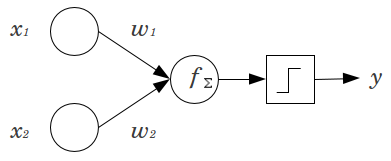
\includegraphics[scale = 0.6]{images/perceptron.png}
    \caption{Perceptron}
    \label{perceptron}
\end{figure}

%\begin{wrapfigure}{r}{5cm}
%\centering
%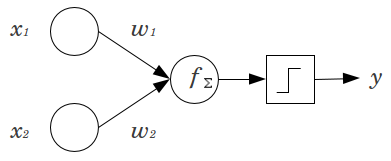
\includegraphics[width = 8cm ]{images/perceptron.png}
%\end{wrapfigure}

Le perception est un réseau de neurone artificiel à une couche d'entrée et une de sortie sans couche cachée. Comme on peut voir un exemple sur la figure \ref{perceptron}, le perception est le modèle de réseau de neurones le plus simple. Son défaut est son incapacité à estimer une fonction non linéaire.\\


\begin{itemize}
    \item \textbf{Perception multi-couches (MLP)}
\end{itemize}


%\begin{wrapfigure}{r}{5cm}
%\centering
%\rule{3cm}{7cm}
%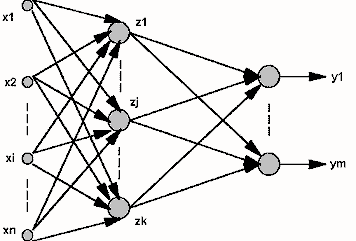
\includegraphics[width = 8cm ]{images/multicouche.png}
%\end{wrapfigure}

Le MLP(Multi-layer perceptron) est un réseau de neurones à au moins une couche cachée. On peut le considérer comme une séquence d'un ensemble de perceptrons. Cette manière de séquencer les perceptrons et d'activer chaque sortie de chaque percetron par une fonction non linéaire émerge un comportement non linéaire permettant ainsi d'estimer les fonctions non linéaire. Le nombre de séquence de perceptron défini la profondeur de l'architecture du réseau. Le MLP augmente le nombre de paramètres(poids) à calibrer, en fonction de l'augmentation de la profondeur. L'augmentation de la profondeur peut facilement amener le modèle à spécialiser le calibrage des poids sur les données d'entrée (sur-apprentissage), ce qui entraîne une mauvaise estimation d'un nouveau exemple.  
\begin{figure}[H]
    \centering
    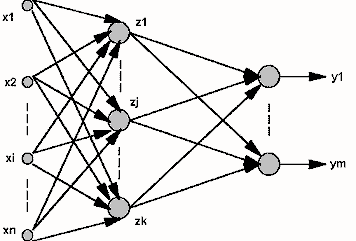
\includegraphics[scale = 0.5]{images/multicouche.png}
    \caption{MLP}
    \label{mlp}
\end{figure}

%\subsection{Réseau de neurones récursifs}
%Le réseau de neurones récursifs est un des modèles de réseau de neurones doté d'une %capacité de mémorisation grâce à son système de récursion et est adapté aux données à %évolution temporelle. Il est très utilisé dans le traitement des langages. Il souffre %énormément de la perte du gradient et de l'explosion de ce dernier. LSTM est un type de %réseau de neurones récursifs permettant de surmonter ce problème.
\subsection{Auto-Encoder}
%\begin{wrapfigure}{r}{4cm}
%\centering
%\rule{3cm}{7cm}
%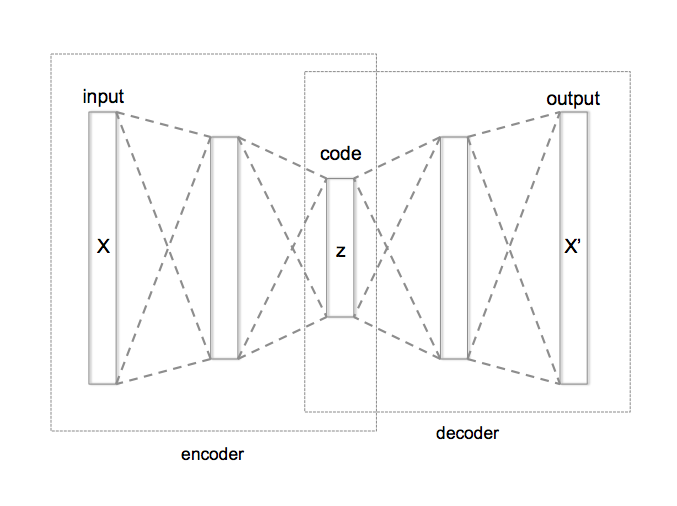
\includegraphics[width = 8cm ]{images/Autoencoder_structure.png}
%\end{wrapfigure}
Un auto-encoder est un réseau de neurones dont sa phase d'apprentissage est non supervisée et chaque sortie du réseau est semblable à l'entrée. Le vecteur résultant est l'une des couches cachée appelée le code qui est un condensé de la représentation de l'entrée, il est comme l'analyse de la composante principale (PCA) mais il permet de plus une représentation non linéaire par rapport au PCA \cite{ann1}. La partie de l'architecture réseau avant l'obtention du code est appelé codeur et celui après le décodeur, comme on le voir sur la figure \ref{autot_encoder}.
\begin{figure}[H]
    \centering
    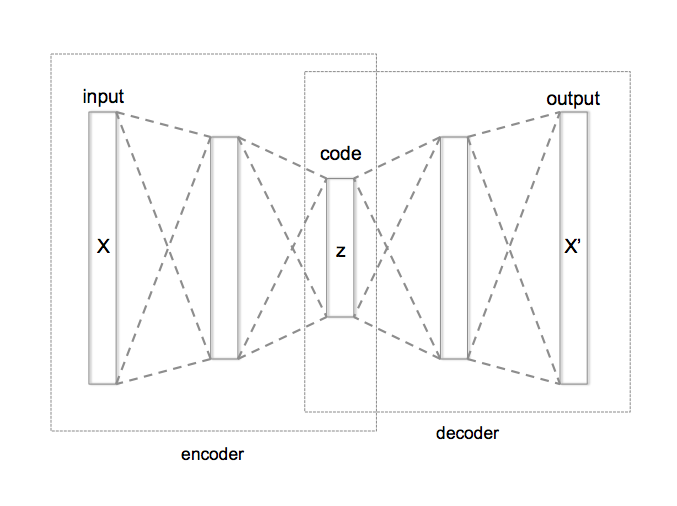
\includegraphics[scale = 0.4]{images/Autoencoder_structure.png}
    \caption{Auto-encoder}
    \label{autot_encoder}
\end{figure}

\section{Réseau de neurones convolutifs (CNN)}
Les réseaux de neurones convolutifs sont de type de réseau de neurone travaillant sur des images en se focalisant sur des caractéristiques locaux de l'image qu'il transforme d'une abstraction à une autre à travers les couches \cite{adavencedCNN}. Il s'inspire du cortex visuel du chat, ce qui le rend plus approprié pour la vision artificielle.\\

Le réseau convolutif permet non seulement l'obtention d'une bonne précision par rapport au réseau de neurone classique mais aussi permet la diminution du nombre de paramètre du réseau à apprendre (les poids) à travers le partage des poids.\\

\textbf{Noyau ou filtre(Kernel), Opération de convolution, Déplacement (strides),  Padding } \\%\cite{}\\
Le noyau est la matrice de paramètres qui se connecte sur la partie locale de l'image pour l'opération de convolution, donc cette partie locale doit avoir la même dimension que le noyau. Le noyau contient alors les paramètres (poids) à apprendre et il sera utilisé pour tout le reste des parties locales de même taille de l'image en faisant passer une fenêtre de déplacement sur l'image. L'opération de convolution est de multiplier case par case les deux matrices pour obtenir une matrice M, puis faire la somme des éléments de M pour l'obtention d'un scalaire qui est le résultat final de la convolution, c'est donc une fonction non inversible. Le déplacement est le nombre de case pour se déplacer vers la droite et en bas pour positionner le noyau sur une nouvelle partie locale de l'image pour une autre opération de convolution. Au coin supérieur gauche de l'image la position du  déplacement est (0,0), puisque une opération complète de convolution donne comme résultat une image intermédiaire A qui est une abstraction de l'ancienne, la valeur de A(i,j) correspond au résultat de l'opération de convolution à la position du déplacement (i,j).À la position (p, q) de déplacement, la prochaine position à droite est (p+1, q) et en bas (p, q+1). On remarque rapidement la diminution de la dimension de l'image , le padding permet d'augmenter la taille de l'image par des zéros pour avoir la même dimension de sortie que l'entrée.\\


\textbf{Fonctionnement}\\
Le réseau convolutif divise la matrice de l'image en des petites matrices(de même taille que le noyau) ordonnées par leurs positions et ces petites matrices passe dans le même réseau de neurones (c'est-à-dire les mêmes poids : noyau) pour donner une nouvelle matrice en sortie qui sera à son tour une entrée d'une nouvelle couche et ainsi de suite jusqu'à la sortie. Dans mon explication ci-dessus certes j'ai fait plus d'abstraction de certains détails, il y a pas que de couches de convolution qui existe, il y à des couches de regroupement (pooling), de couches d'activation (ReLu (généralement utilisé), softMax, tanh, ...), de couche de simplification pour empecher de passer en surapprentissage (dropout, batch normalization, ...) \cite{adavencedCNN}

\begin{figure}[H]
    \centering
    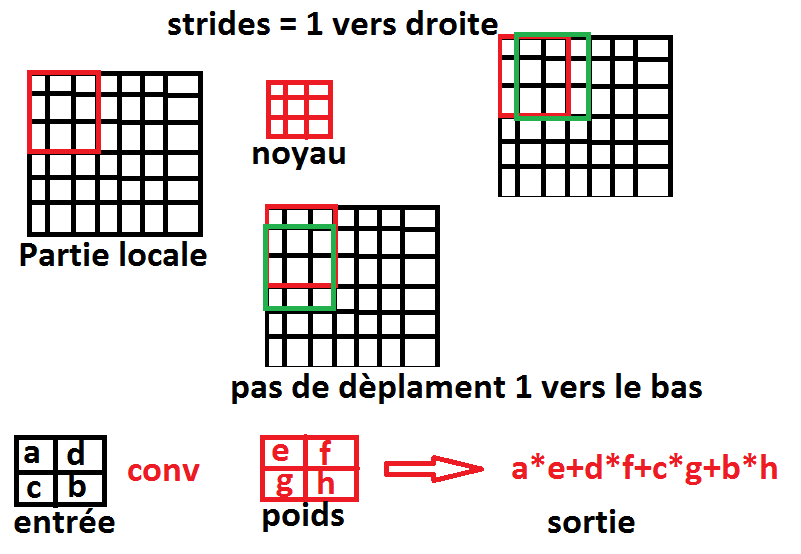
\includegraphics[scale = 0.7]{images/operations_conv.png}
    \caption{fonctionnement du réseau de neurone convolutif}
\end{figure}

\subsection{Couche convolutive}
Plusieurs amélioration de la couche convolutive ont été proposées dans la littérature et ont donné des bons résultats surtout sur la base de données de Image-Net \cite{im1}%plusieurs à cité
Nous avons plusieurs de réseau convolutifs, mais nous avons présenter que quelques en détail.
\begin{figure}[H]
    \centering
    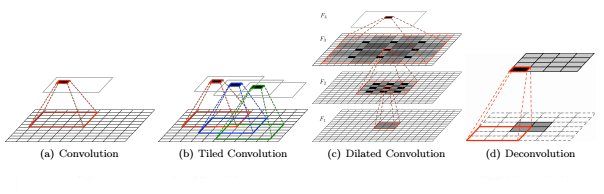
\includegraphics[scale = 0.8]{images/all_cnn.png}
    \caption{Illustration de quelques type de CNN}
\end{figure}
\subsubsection{Tiled convolutional network (TCN)}
Le réseau convolutif d'origine n'utilise qu'un seul noyau qui est partagé entre toutes les parties locales de l'image. Il permet d'éviter des problèmes de translation mais pas d'autres dérangement dans l'image telle la rotation. Le TCN permet d'utiliser à chaque couche convolutive plusieurs noyaux, ainsi permettant plus d'abstractions\cite{tcnn1, tcnn2, tcnn3}. 



\subsubsection{Transposed convolution ou Deconvolution (TC)}
Une couche convolutive de CNN prend une image (matrice) en entrée et retourne une autre image de dimension inférieur ou égale à l'image d'origine, le TC fait l'opération inverse. Le TC transforme chaque case de la matrice de l'image en une petite matrice. Ce n'est pas vraiment une opération inverse du CNN comme l'apparence nous fait croire mais c'est juste le type d'entrées et sorties qui sont inversé. Pour un CNN, les poids se fixent sur une localité et retourne un scalaire tandis pour TC on part d'un scalaire pour arriver à une matrice locale. Pour plus de détail on peut voir \cite{transcd1, transcd2, transcd3,transcd4, transcd5}  
\subsubsection{Dilated convolutional neural}
Le dilated convolution neural élargit de plus le filtre en mettant autant des zéros que nécessaires (un hyper-paramètre à donner) entre une case et ses voisines de la matrice noyau. Pour plus de détail concernant le dilated convolutional le lecteur peut se référer \cite{dilate1, dilate2, dilate3, dilate4}.
\subsubsection{Network in network (NiN)}
Le NiN\cite{nin1} est une des améliorations la plus intéressante par rapport aux précédentes, elle permet dans chaque couche convolutive d'utiliser comme filtre un petit réseau de neurones profonds. C'est-à-dire sur la partie locale, est appliquée un petit réseau de neurones profond au lieu d'un perceptron comme dans le cas du CNN. C'est qui veut dire qu'une couche de NiN est constituée d'une couche de convolution de noyau (k, m) suivi par plusieurs couches de convolution de noyau (1,1) chacune.

\begin{figure}[H]
    \centering
    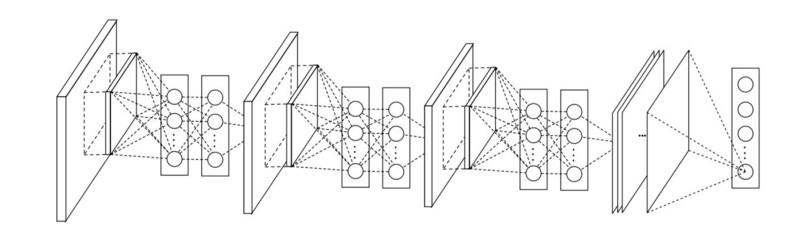
\includegraphics[scale = 0.5]{images/nin.jpg}
    \caption{Illustration NiN}
\end{figure}
\subsubsection{Inception module}
Inception module\cite{im1, im2, im3, im4} est une généralisation de NiN, dans chacune de ses couches on peut avoir plusieurs successions de couches convolutives de noyau de dimension (k$_i$,m$_i$) où les (k$_i$,m$_i$) ne sont pas nécessairement des couples de 1, les résultats de cet ensemble de couches successives sont fusionnés pour donner un ensemble d'images qui sont plus d'abstraction (profondeur). Un type de ce modèle a gagné le prix du challenge de la reconnaissance visuelle sur ImageNet en 2015 (GoogleNet \cite{im1}). Plusieurs amélioration de ce modèle ont été fait, il y a eu même une fusion avec le residual network qui donne plus de précision et permet de réduire le temps d'apprentissage également \cite{im1, im2, im3, im4}. Notre modèle s'inspire de ce type de réseau convolutif. 

\begin{figure}[H]
    \centering
    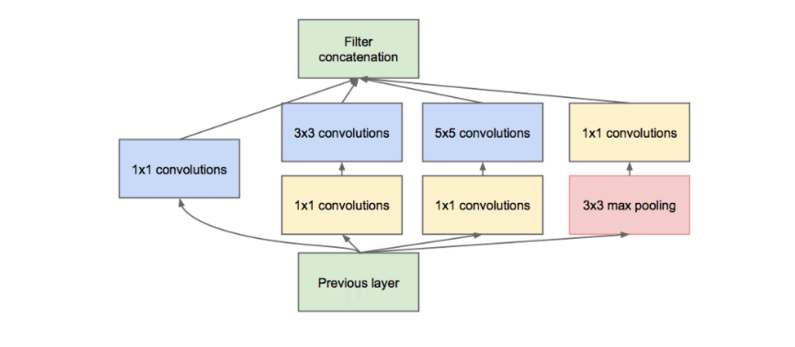
\includegraphics[scale = 0.5]{images/im.png}
    \caption{Illustration Inception module}
\end{figure}

%\subsubsection{Residual convolutional neural network}
\subsection{Couche d'agrégation (pooling)}
La couche d'agrégation permet non seulement la réduction de la dimension mais également permet de capturer certaines abstractions statistiques locales \cite{pool1, pool2, pool3, pool4}. Plusieurs couches d'agrégation ont été définies parmi elles la couche maxpooling et celle de averagePooling sont les plus utilisées. La couche maxpooling permet de choisir la valeur maximale locale parmi les valeurs de la région considérée et le averagepooling fait la moyenne de la région locale considérée.

\begin{figure}[H]
    \centering
    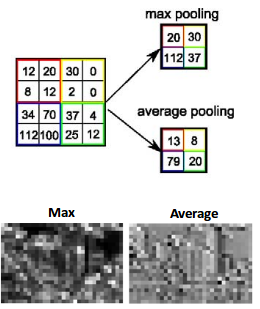
\includegraphics[scale = 0.5]{images/average_max.png}
    \caption{maxpooling et averagepooling}
\end{figure}


\section{Boosting}\label{section22}
Le boosting est une technique d'apprentissage qui s'appuie sur des modèles légers appris pour construire de modèles sophistiqués. Il opère de manière séquentielle d'un modèle à un autre tout en corrigeant l'erreur du précèdent en augmentant la distribution de ceux qui sont mal prédits. L'ensemble des modèles légers n'est pas nécessairement homogène, on peut faire le boosting avec plusieurs modèles de familles différentes. Ce type de modèle ne cessent de nous surprendre dans certains domaine par rapport aux réseaux de neurones profonds comme dans notre étude actuelle.

\textbf{Regularized gradient boosting tree}\\
Un arbre de décision est une fonction/modèle permet d'estimer une valeur ou classifier en construisant un arbre dont les feuilles sont les classes ou les valeurs estimées. Formellement un arbre de décision est décrit comme suit: \\ Soit $x \in R^n$ l'objet pour lequel une valeur y doit être prédite, $f$ la fonction correspondant à l'arbre de décision.
$f(x) = W_{q(x)}$ où $W \in R^d$  est le vecteur correspondant aux valeurs prédites et $q: R^n -> \{1..d\}$.

gradient boosting tree est la version du boosting où le modèle léger est un arbre de décision et l'ensemble de ces modèles est obtenu en minimisant le gradient, du passage d'un modèle à un autre. Pour éviter le problème du sur apprentissage, les techniques de régularisation sont appliquées. Supposons que nous avons $k$ estimateurs (modèles légers appris), l'estimation d'une valeur correspondante à $x$ est $\widehat{y} = \sum \limits_{i=1}^k f_i $ 

Le problème d'optimisation se résume à minimiser l'expression suivante : \\
$L(\Phi) = \sum \limits_{i=1}^n l(y, \widehat{y}) + \sum \limits_{j=1}^k \Omega(f_j)$ où $l(y, \widehat{y})$ est la fonction de perte, $\Omega(f_j)$ permet de contrôler la complexité du modèle pour empêcher le sur-apprentissage et $\Phi$ est l'ensemble de paramètres. $\Omega(f_j) = \frac{1}{2} \lambda \sum \limits_{i=1}^m W_{i}^2 + \alpha\sum \limits_{j = 1}^m |W_j| + \gamma m$, où $\lambda$, $\alpha$ et $\gamma$ sont des hyper-paramètres. \\Son implantation est xbboost, pour plus de détails on peut se référer cite{boost}.

\section{Apprentissage profond}
Le problème d'apprentissage se résume à un problème d'optimisation, çà revient à adapter les paramètres du modèle pour une généralisation du monde concerné (population) à partir d'un échantillon des données. L'apprentissage profond est l'adaptions des paramètres d'un modèle construit à partir de la superposition de plusieurs couches de réseau de neurones. La Superposition des couches permet de capturer plus d'abstractions. Ces paramètres sont appelés les poids (weights) du réseau.
\subsection{Apprentissage par rétro-propagation}
La rétro-propagation permet de propager l'erreur en arrière sur toutes les couches pour ajuster les poids.
\subsubsection{Optimisation}
Trouver les poids adaptés se ramène à optimiser une certaine fonction. Cette fonction dépend du type d'architecture de réseaux de neurones. La prédiction d'un individu X par une architecture de n couches en mode feed foward ou une architecture où les signes sont propagés dans un seul sens de l'entrée à la sortie (comme MLP) est $\widehat{Y} = Y_n$ tel que $Y_1 = \sigma(W_1*X + b_1)$, $Y_2 = \sigma(W_2*Y_1 + b_2)$, $... Y_n = \sigma(W_{(n-1)}*X + b_{(n-1)})$ où $W_i$ sont les poids du réseaux, $b_i$ les biais et $\sigma$ la fonction d'activation \cite{relu, rnna, erc}. Pour l'obtention des poids adaptés d'une architecture feed forward, il revient à minimiser la fonction $\sum \limits_{i=1}^m L(Y^i, \widehat{Y}^i)$ où $Y^i$ est la vraie valeur correspondante à X, m est la taille de l'échantillon et $L$ est la fonction de perte ainsi dans notre cas $L(Y, \widehat{Y}^i) = (\frac{Y-\widehat{Y}}{Y+1})^2$. Pour la minimisation, la descente du gradient est utilisée, pour chaque étape du gradient les paramètres et biais sont mis en jours. $W^i = W^{i-1} - \alpha \frac{\delta L}{\delta W} W^{i-1}$ où $\alpha$ est le taux d'apprentissage .\\

Le problème majeur du gradient est la difficulté d'obtention du minimum global, la rapidité de convergence et son coup de calcul. Plusieurs améliorations du gradient ont été effectuées concernant ces problèmes (SGD \cite{sgd_}, AdaGrad \cite{adagrad}, Adam \cite{adam}, ...). Pour ce travail Adam et SGD ont été utilisés.


\subsubsection{Régularisation}
La régularisation permet de contrôler la complexité du modèle en pénalisant la fonction à optimiser d'une certaine valeur. Ce qui permet au modèle de généraliser mieux le monde concerné et éviter le sur apprentissage. Plusieurs méthodes de régularisations existent:
\textbf{Batch normalisation \cite{batch}} qui normalise les données à l'entrée de la couche suivant la couche du batch, \textbf{L1 et L2} qui augmente sur la fonction de paramètres à optimiser la quantité respectivement $\lambda * \sum \limits_{i = 1}^m |w_i|$ et  $\lambda * \sqrt[\,] {\sum \limits_{i = 1}^m w_i^2} $)
 où $\lambda$ est un hyper-paramètre, et dropout qui supprime certains neurones d'une certaine proportionnalité $\alpha$ de la couche concernée. Dans ce travail batch normalisation, L2 et dropout ont été utilisés.

\chapter{Résultats et discussion}

\section{Données}
Dans cette section, nous allons décrire les pré-traitement sur les données (images) et mentionner leur source ainsi que le mode d'accès.
\subsection{Source et nature de données}

\subsubsection{SDSS(Sloan Digital Sky Survey IV)}
En termes simples, le Sloan Digital Sky Survey est l'étude astronomique la plus ambitieuse jamais entreprise. SDSS a observé en détail un quart de l'ensemble du ciel, déterminant les positions et la luminosité absolue de centaines de millions d'objets célestes\cite{sdss}. Il mesure également les distances à plus d'un million de galaxies et quasars\footnote{http://skyserver.sdss.org/dr13/en/sdss/sdsshome.aspx}. 

\subsubsection{DR13 (database release version 13)} \footnote{http://skyserver.sdss.org/dr13/en/help/browser/browser.aspx}
Data Release 13 stocke les prèmieres données de la quatièmes phase de la collecte de SDSS. Elle inclut les données prises à partir du 25 juin 2015, et englobe plus que un tiers de la sphère céleste. Avec plusieurs mesures du ciel faites et dans plusieurs façons, $1 231 051 050$ objets (catalogues) ont été collectés \footnote{http://www.sdss.org/dr13/scope/} 

\begin{figure}[H]
    \centering
    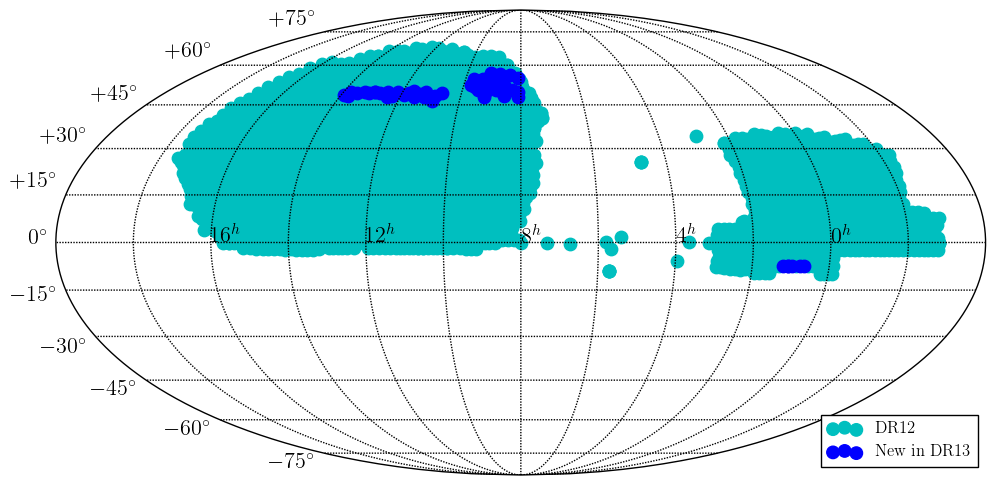
\includegraphics[scale = 0.5]{images/dr13_boss.png}
    %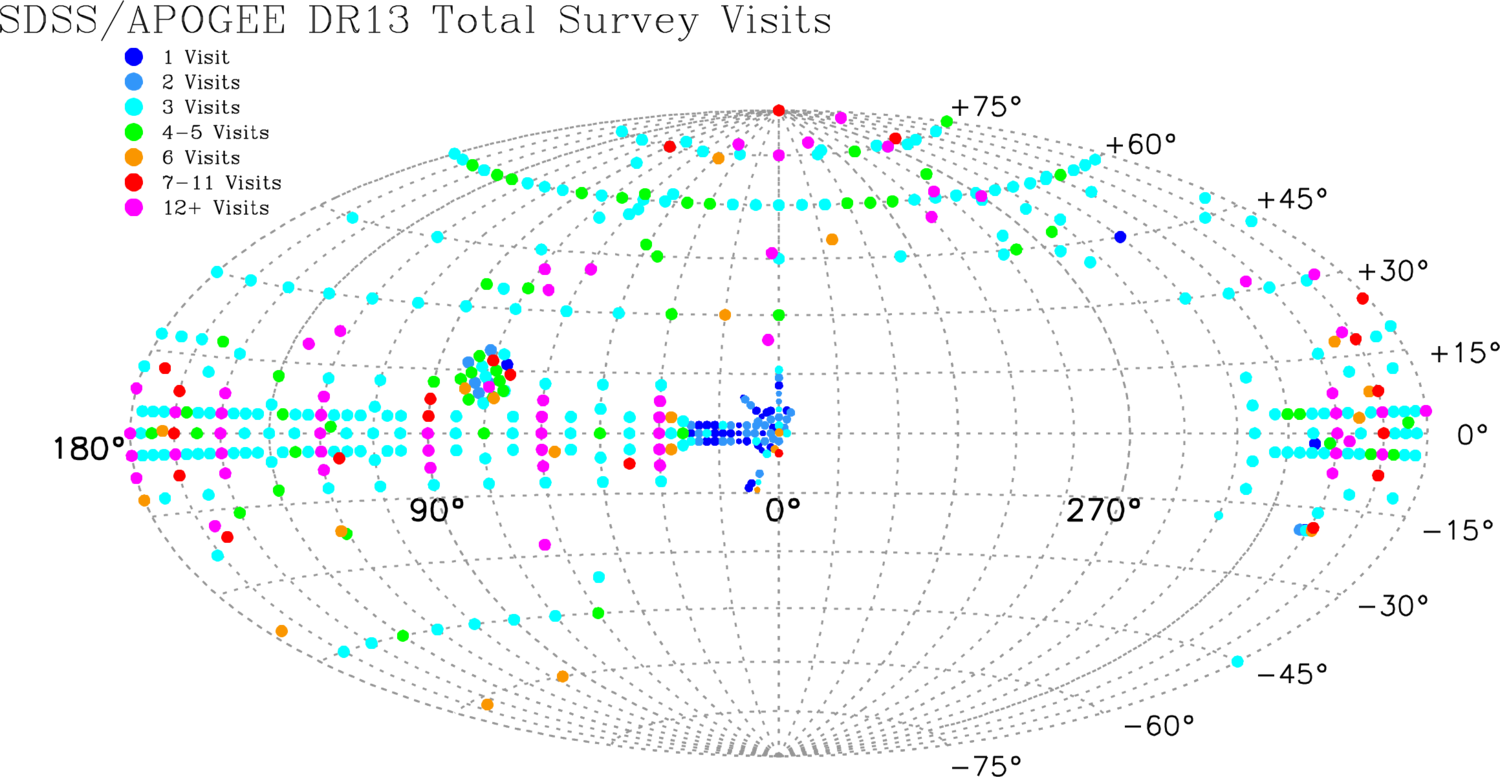
\includegraphics[scale = 0.3]{images/appoge.png}
    %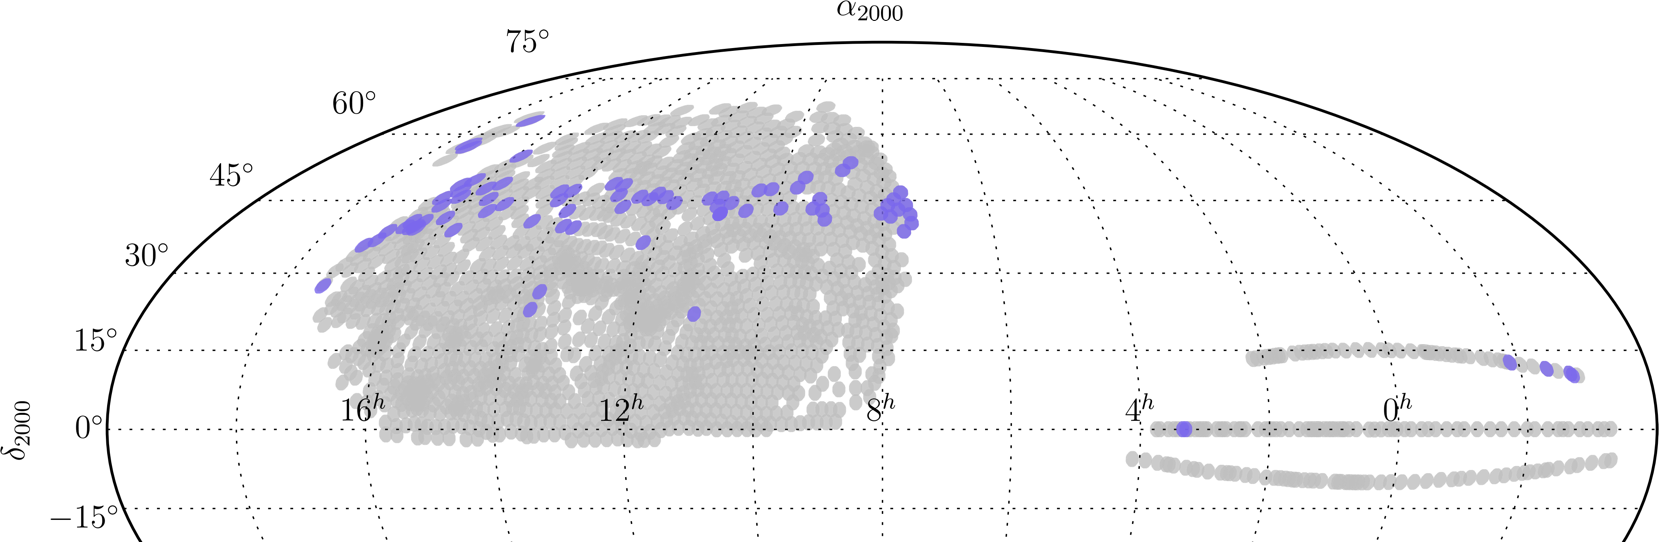
\includegraphics[scale = 0.1]{images/manga.png}
    \caption{eBOSS surveys}%, APOGEE surveys, and MaNGA surveys respectivement de gauche vers droite}
\end{figure}

Toutes nos données proviennent de la collecte de données SDSS . Elles sont télé-chargées sous forme des vecteurs chacune dans 5 bandes différentes (griuz). À partir de ces données sous forme de vecteurs provenant des tables SpecPhoto et PhotoPrimary de DR13 de SDSS, les urls des images correspondant à chaque vecteur sont générés. À partir de ces urls, les images sont télé-chargées et sauvegardées localement. \\

Les données ne sont pas sélectionnées, elles sont chargées directement aleatoires et sont de distributions différentes.
\begin{figure}[H]
	\centering
	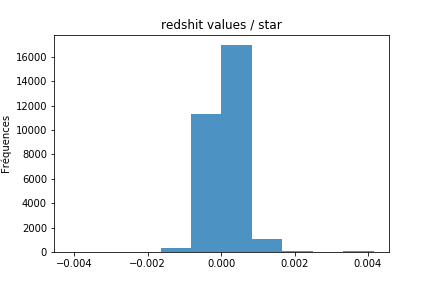
\includegraphics[scale = 0.3]{images/star.png}
	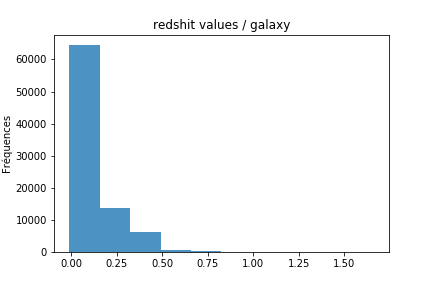
\includegraphics[scale = 0.3]{images/galaxy.png}
	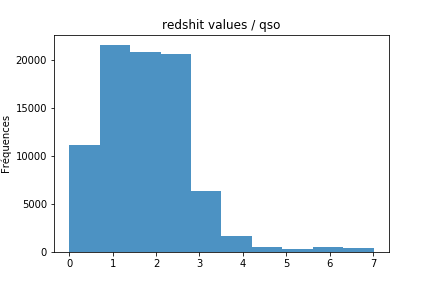
\includegraphics[scale = 0.3]{images/qso.png}
	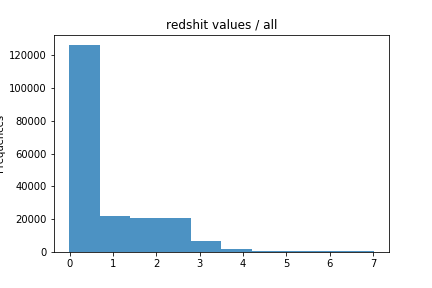
\includegraphics[scale = 0.3]{images/all.png}
	\caption{Distribution du redshift selon les catégories des objets cosmologiques}%, APOGEE surveys, and MaNGA surveys respectivement de gauche vers droite}
\end{figure}

\subsection{Pré-traitement sur les images}
Les images dans leur taille d'origine sont très grandes (1361*2048 pixels), et contiennent des quantités lumineuses très variées.
La taille de chaque image est réduite à 32*32, cette réduction est faite en utilisant la moyenne des coordonnées centrales (rowc$\_$ et colc$\_$) des objets(images) de chaque bande. Pour normaliser, le minimum de la quantité lumineuse (pixel) de chaque image est soustraite de l'image et le logarithme est appliqué à chaque pixel de l'image.  


\begin{figure}[H]
    \centering
    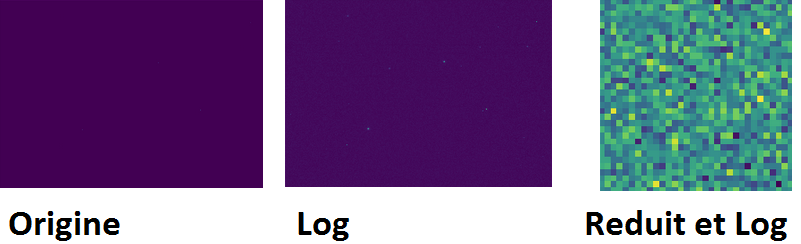
\includegraphics[scale = 0.5]{images/pretaitemen.png}
    \caption{pretement sur les images}
\end{figure}

\section{Configurations techniques}
Pendant toutes nos expérimentations, nous avons utilisés des machines hpc (haute performance computing) équipées d'une carte graphique graphique du type  NVIDIA GP104GL et un processeurs de 10 cœurs physiques de type Intel(R) Xeon(R) CPU E5-2640 v4 avec une fréquence de 2.40GHz.

Pour la concrétisation de notre architecture du CNN, nous avons utilisé la bibliothèque Keras \cite{chollet2015keras}  et pour celle du boosting nous avons utilisé la bibliothèque xgboost \footnote{http://xgboost.readthedocs.io} et scikit-learn \cite{scikit-learn}.
\section{Expérimentations}
Dans ce travail, nous avons choisi d'utiliser deux principales modèles de l'apprentissage automatique à savoir boosting qui est un modèle ensembliste, et réseau de neurones convolutifs (apprentissage profonds). En effets le boosting et les réseaux convolutifs ont donnée des bons résultats non pas seulement sur l'estimation du redshift \cite{meuphirim, isanto} mais également sur d'autres problèmes de régression et classification \cite{boost, adavencedCNN}. \\

Le choix et l'adaptation des hyper-paramètres ont été fait manuellement pour les deux types de modèles en faisant des test sur un petit échantillon de données et quelques combinaisons des hyper-paramètres. Au niveau du CNN, l'obtention des bons hyper-paramètres est compliquée car le CNN possède beaucoup d'hyper-paramètres à adapter.

Dans le tableau tab. \ref{quantite} est mentionnée la taille de données d'apprentissage et test de chaque type de corps cosmologiques.
\begin{table}[H]
	\centering
	\begin{tabular}{|l|l|l|}
		\hline
		$Type\_cosmologique$ & $\#Apprentissage$ & $\#Test$\\
		\hline
		Galaxie &  59887 & 25667\\
		\hline
		Quasar & 58668 & 25144\\
		\hline
		Étoile & 20994 & 8998 \\
		\hline
		Tous & 139550 & 59808 \\
		\hline
		%\hline		
	\end{tabular}
	\caption{Nombre d'élément de chaque type cosmologique}
	\label{quantite}
\end{table}


\subsection{CNN (type: inception module)}
Notre modèle final du type de réseau de neurones, celui qui s'adapte bien à nos données c'est-à-dire qui réduit mieux l'erreur normalisée ($\Delta z_{norm}$) est un réseau convolutif de la famille des inceptions modules. Notre modèle est construit comme suit: \\ Notre couche principale ($cp$) fig.\ref{archi_neural} est constituée de la concaténation de trois sous couches suivies par une sous couche d'agrégation de filtre 2 par 2 et d'un pas de déplacement 2 (strides = 2). Les trois sous couches concaténées sont décrites comme suit:
\begin{itemize}
	\item[$1^{er}$.] Constitué de trois sous couches de convolution de filtre 1*1 et de pas déplacement 1*1 formées de manière séquentielle.
	\item[$2^e$] Trois sous couches de convolutions formées de manière séquentielle de 3*3 comme filtre et de 1*1 comme pas déplacement.
	\item[$3^e$] Trois sous couches de convolution formées de manière séquentielle de 5*5 comme filtre et de 1*1 comme pas déplacement.
\end{itemize} 
\begin{figure}[H]
	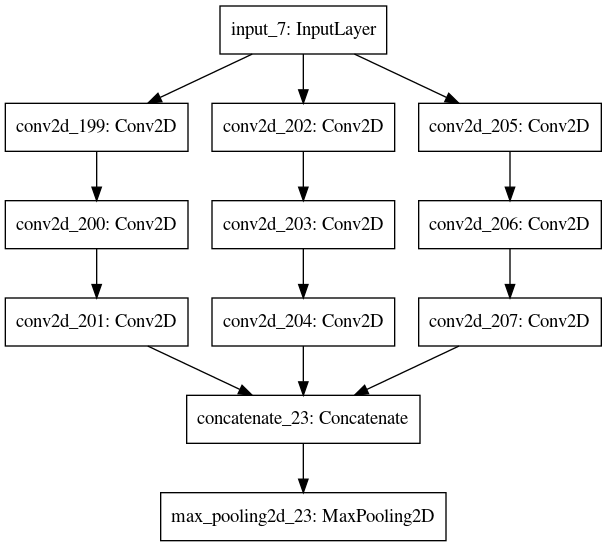
\includegraphics[scale = 0.5]{images/kernel.png}
	\caption{La couche principale de notre architecture neurale}
	\label{archi_neural}
\end{figure}
Dans chaque couche convolutive, la fonction d'activation est $relu(x) = max (0, x)$, pour éviter le sur-apprentissage une régularisation de type $l2$ est appliquée à chaque couche convolutive. Le padding zéro est appliqué sur toutes les couches convolutives. Notre architecture finale est constituée de 5 couches du même type que la $cp$ avec de nombre des sorties différents. Pour l'apprentissage, $Adam$ est utilisé entant qu'algorithme d'optimisation, à chaque deux reprises (epochs) de l'algorithme le taux d'apprentissage est divisé par deux, le early stoping est appliqué pour éviter le sur apprentissage de plus. Le early stoping est une manière d'arrêter rapidement l'apprentissage quand la précision sur les données d'apprentissage est sur le point de dépasser celle sur les données de validation. Le nombre de reprise(epochs) est paramétré à 30 et la taille de batch size est mise à 256.

Dans la suite du document, nous supposons les conventions suivantes:
$out1 = |znorm| > 0.15 (\%)$,  $out2 = |znorm| > 3std (\%)$, $RZ = RMSE\_znorm$ 
%\subsection{Expérimentions avec CNN}
\begin{table}[H]
	\centering
	\begin{tabular}{|l|l|l|l|l|l|l|}
		\hline
		type & $RZ$ & $\mu_{norm}$ & $\sigma_{norm}$ & RMSE & $out1$ & $out2$ \\
		\hline
		GXY/CNN & 0.035056 & 0.035032 & 0.035032 & 0.046099 & 0.752123 & 1.310150 \\
		\hline
		QSO/CNN & 0.289760 & 0.276163 & 0.276163 &1.065627 & 66.988385 & 0.441682\\
		\hline
		All/CNN & 0.261338 & 0.252728 & 0.252728 & 0.906072& 34.453168 &1.325543 \\
		\hline
		%\hline		
	\end{tabular}
	\caption{Résultats du CNN}
\end{table}

Ces résultats s'éloignent, dans le sens négatif, des meilleurs résultats de l'état de l'art. Cette mauvaise estimation de redshift par notre architecture de réseau convolutif peut s'expliquer par plusieurs raisons dont le fait qu'on possède moins de données pour booster l'apprentissage, le fait que l'image est trop réduite (trop de perte d'information) sans essayer de la réduire par la convolution.
 
\subsection{Boosting (type: xgboost)}
Trois principaux hyper-paramètres (nombre d'estimateurs, taux d'apprentissage et la profondeur de l'arbre) ont été réglés et adapté et tout le reste des paramètres ont été laissé avec leurs valeurs par défaut. Les trois modèles configurés du boosting sont mentionnés dans le tableau \ref{param_boost}.\\
\textbf{Quelques paramètres commun}\\
learning\_rate = 0.1, colsample\_bylevel=0.592, reg\_alpha=0.651, reg\_lambda=2.84
\begin{table}[H]
    \centering
    \begin{tabular}{|l|l|l|}
         \hline 
         modèles&n\_estimators&max\_depth\\
         \hline
          model1 &150&6\\
         \hline
         model3&150&5\\
         \hline         
         model2 &200&5\\
         \hline
         %mod1&&&&&&&
         %\hline
    \end{tabular}
    \caption{Paramètres de différents modèles de xgboost}
    \label{param_boost}
\end{table}

%\section{Résultats}


\subsection{Expérimentions avec XGBoost}
\begin{table}[H]
	\centering
	\begin{tabular}{|c|l|l|l|l|l|l|l|}
		\hline
		model & type & RMSE\_znorm & $\mu_{norm}$ & $\sigma_{norm}$ & RMSE & $out1$ & $out2$ \\
		\hline
		%\multirow{2}{1cm}{$model1$}& & & & & & \\
		
		\multirow{2}{1cm}{$model1$} & Galaxy  & 0.035728 & 0.000548 & 0.035723 & 0.046813 & 0.654537 & 1.137648 \\
		%\hline
		\cline{2-8}
		 & QSO & 0.318635  & 0.017468  & 0.318156  & 0.940743 & 64.03118 & 0.898823 \\
		 %\hline
		 \cline{2-8}
		 & All & 0.320223  & 0.015833  & 0.319832  & 0.801991 & 38.971375 & 2.543138 \\
		 %\hline
		 \cline{2-8}
		 & Star & 0.000429 & 0.000015  & 0.000428  & 0.000429 & 0.0       & 1.066904 \\
		 
		\hline
		\multirow{2}{1cm}{$model3$} & Galaxy  & 0.035938 & 0.000375 & 0.035936 & 0.04507 & 0.580512 & 1.133752 \\
		%\hline
		\cline{2-8}
		& QSO & 0.318635 & 0.017468 & 0.318156 & 0.940743 & 64.03118 & 0.898823 \\
		%\hline
		\cline{2-8}
		& All & 0.31818 & 0.010996 & 0.31799 & 0.799093	& 39.24057  & 2.539794 \\
		%\hline
		\cline{2-8}
		& Star & 0.000432 & 0.000013 & 0.000432 & 0.000433 & 0.0    & 1.044677 \\
		
		\hline
		\multirow{2}{1cm}{$model2$}& Galaxy & 0.03556 & 0.000058 & 0.03556 & 0.046432 & 0.654537 & 1.211673\\
		\cline{2-8}
		& QSO & 0.317182 & 0.016874 & 0.316733  & 0.957897	& 64.528317  & 	0.775533 \\
		\cline{2-8}
		& All & 0.320004 & 0.013142 & 0.319734 & 0.798689 & 39.569957 & 2.523074 \\
		\cline{2-8}
		&Star& 0.000423 & 0.000011 & 0.000423 & 0.000423 & 0.0 & 1.044677 \\
		\hline		
	\end{tabular}
	\caption{Résultats du XGBoost }	
\end{table}

Les résultats obtenus par xgboost sont intéressants et s'approchent mieux des ceux existants dans l'état de l'art \cite{meuphirim, isanto, photoredSDSS}. Nous remarquons que les modèles estiment bien les objets qui sont proches comme les étoiles puis les galaxies. Pour une estimation non biaisée tous les types de corps cosmologiques sont considérés et le modèle réduit mieux l'erreur sur l'ensemble de ces données fusionnées. 




















%\part{Supernovae classification by time series}
%\section*{Context and motivation}
\section*{Transcient}
\section*{supernovae}
%\chapter {La classification des Supernova dans la littérature}

%\chapter{Description de Données}
%\chapter{Différentes méthodes de classification de séries temporelles}
%\include{experiments}



\chapter*{Conclusion et perspectifs}

\chapter*{Appendix}
\chapter*{Appendix}
\subsection*{Différentes requêtes}
\subsubsection*{Pour les Galaxies}
\noindent SELECT TOP 200000\\
p.objid, s.rowc\_u, s.rowc\_i, s.rowc\_z, s.rowc\_g, s.rowc\_r, s.colc\_u, s.colc\_i, s.colc\_z,s.colc\_g, s.colc\_r, p.rerun, p.run, p.camcol, p.field, p.z as redshift, p.class \\
FROM SpecPhoto AS p JOIN PhotoPrimary AS s ON s.objid = p.objid\\
where p.class = 'GALAXIES'
\subsubsection*{Pour les Quazars}
\noindent SELECT TOP 200000\\
p.objid, s.rowc\_u, s.rowc\_i, s.rowc\_z, s.rowc\_g, s.rowc\_r, s.colc\_u, s.colc\_i, s.colc\_z, s.colc\_g, s.colc\_r, p.rerun, p.run, p.camcol, p.field, p.z as redshift,p.class \\
FROM SpecPhoto AS p JOIN PhotoPrimary AS s ON s.objid = p.objid\\
where p.class = 'QSO'
\subsubsection*{Pour les étoiles}
\noindent SELECT TOP 200000\\
p.objid, s.rowc\_u, s.rowc\_i, s.rowc\_z, s.rowc\_g, s.rowc\_r, s.colc\_u, s.colc\_i, s.colc\_z, s.colc\_g, s.colc\_r, p.rerun, p.run, p.camcol, p.field, p.z as redshift, p.class\\
FROM SpecPhoto AS p JOIN PhotoPrimary AS s ON s.objid = p.objid\\
where p.class = 'STAR'
\subsubsection*{Codes}
\textit{https://github.com/oussissa123/redshift\_estimation}
\subsection*{Quelques figures}

\begin{figure}[H]
	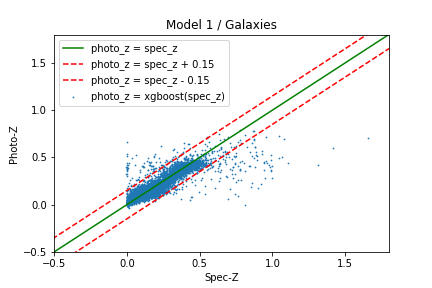
\includegraphics[scale = 0.4]{images/model1_galaxies.png}
	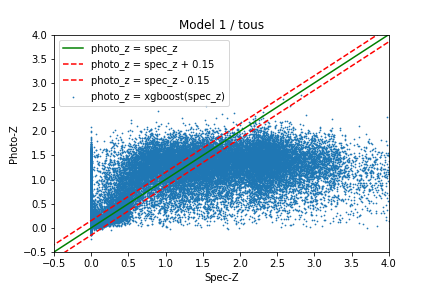
\includegraphics[scale = 0.4]{images/model1_tous.png}
	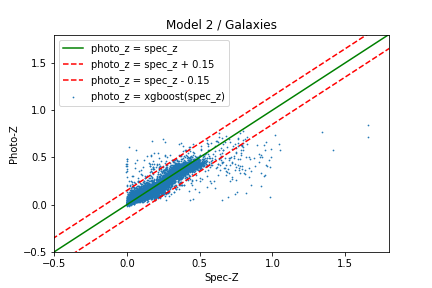
\includegraphics[scale = 0.4]{images/model2_galaxies.png}
	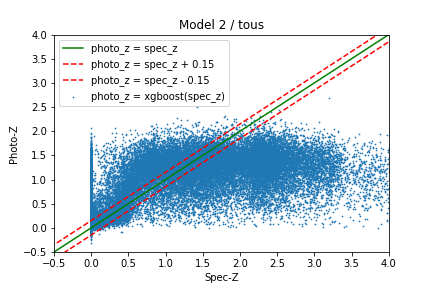
\includegraphics[scale = 0.4]{images/model2_tous.png}
	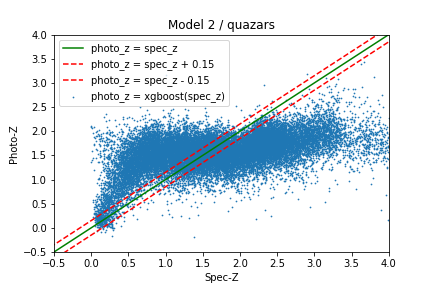
\includegraphics[scale = 0.4]{images/model2_quazars.png}
	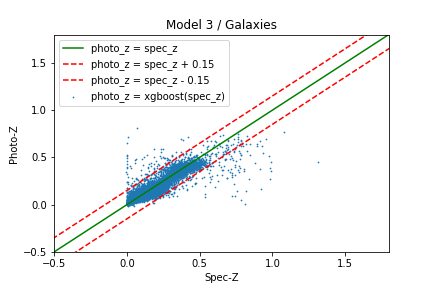
\includegraphics[scale = 0.4]{images/model3_galaxies.png}
	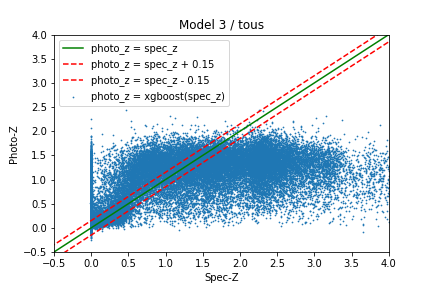
\includegraphics[scale = 0.4]{images/model3_tous.png}
	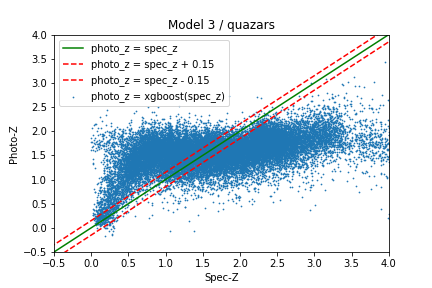
\includegraphics[scale = 0.4]{images/model3_quazars.png}
	\caption{Perturbation entre les valeurs spectroscopiques et photométriques à partir du modèle Boosting sur l'ensemble de test}
\end{figure}



\printbibliography



\end{document}
